\section{Evaluation} \label{sec:Evaluation}
Für die Auswertung der Zuordnungsverteilungen aller Konfigurationen des Versuchssystems werden die Ergebnisse zunächst grafisch dargestellt.
Dabei werden in allen Grafiken die Ergebnisse der drei neuronalen Netze pro Konfiguration miteinander Verrechnet.
Es werden vier verschiedene Aspekte betrachtet (vgl. Abbildung~\ref{fig:AuswertungVersuchssystem}).
\begin{figure}[H]
    \centering
    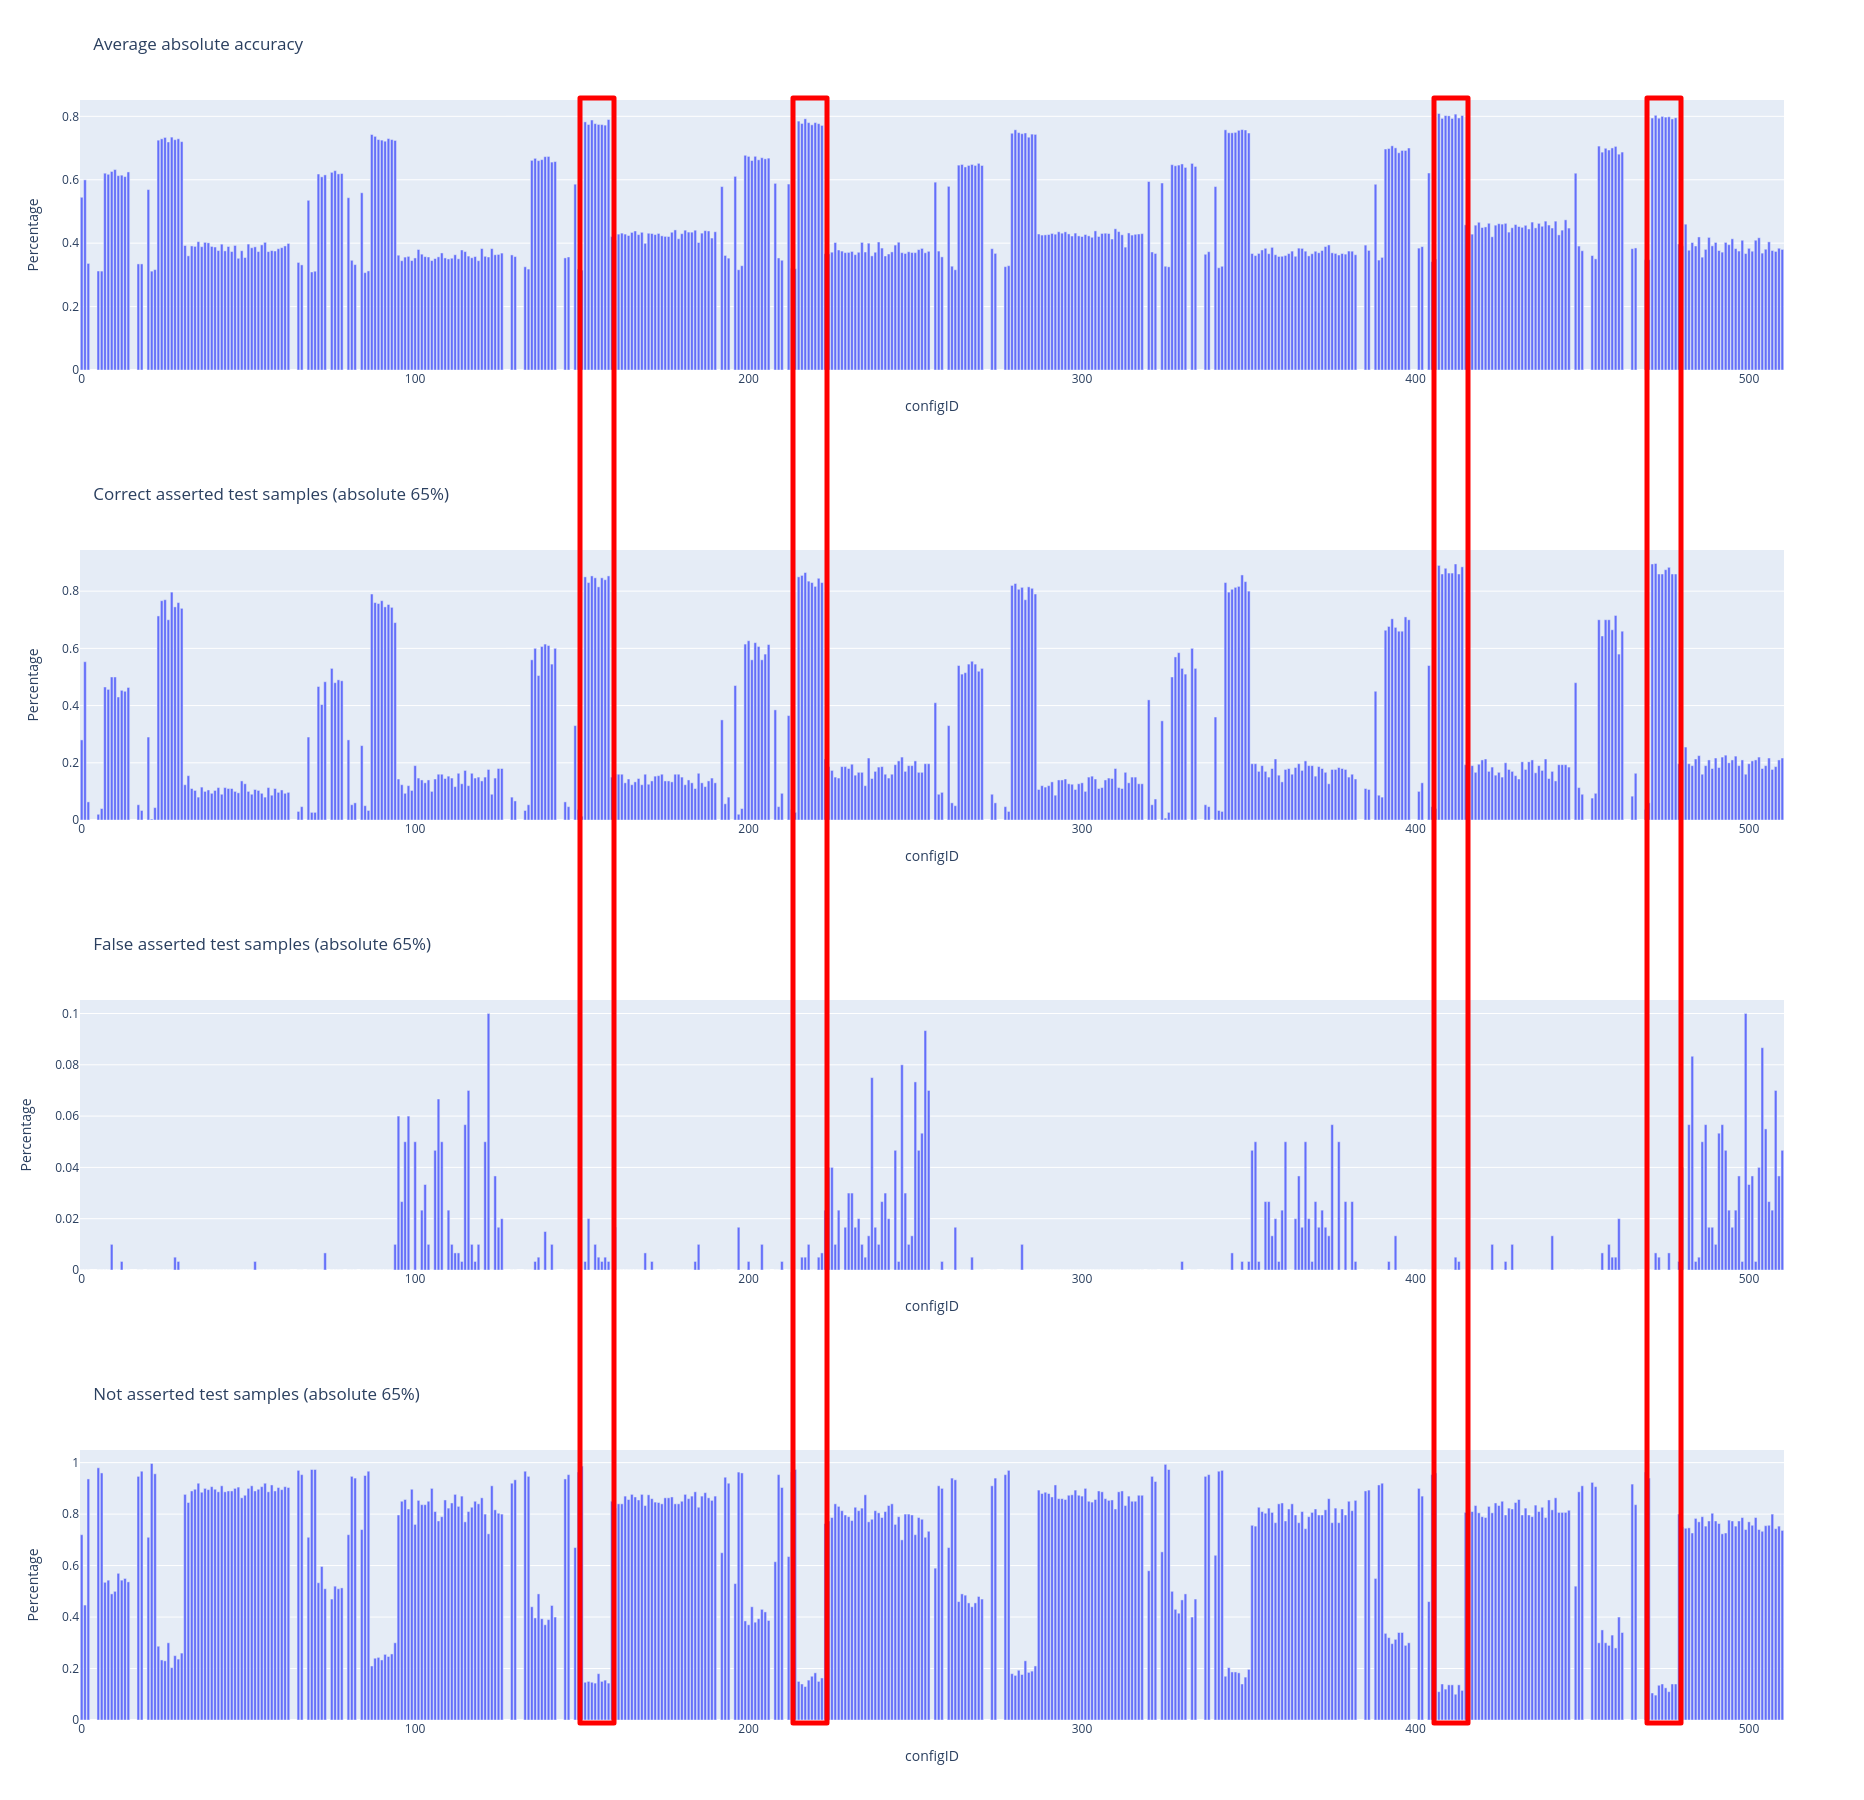
\includegraphics[width=1\textwidth, keepaspectratio]{images/Auswertung.png}
    \caption{Auswertung Versuchssystem}
    \label{fig:AuswertungVersuchssystem}
\end{figure}

Für die durchschnittliche absolute Genauigkeit werden die Wahrscheinlichkeiten für den zu identifizierenden Benutzer pro Testdatei aufsummiert und der Durchschnitt gebildet.
Eine Genauigkeit von 80 \% entspricht damit der Aussage, dass das neuronale Netz in Kombination mit der jeweiligen Konfiguration dem zu authentifizierenden Benutzer im Durchschnitt 80 \% der Frames der Testdatei zuordnet.

Bereits in dieser Grafik zeigt sich die Bildung von Clustern.
Die besten Konfigurationen erreichen eine Genauigkeit von über 65 \%, weshalb dieser Wert für die folgenden drei Auswertungen verwendet wird.
Hier werden die Testdateien mittels dieses Wertes in die drei Kategorien korrekt zugeteilt, falsch zugeteilt und nicht zugeteilt eingeordnet.

Eine Testdatei gilt als korrekt zugeteilt wenn dem zu authentifizierenden Benutzer mindestens 65 \% der Frames zugeordnet werden.
Analog gilt die Testdatei als nicht korrekt zugeteilt, wenn einem anderen Benutzer mindestens 65 \% der Frames zugeordnet werden.
Erreicht kein Nutzer mindestens 65 \%, so wird die Testdatei als nicht zugeteilt eingestuft.

